\documentclass[12pt,a4paper]{scrartcl}

\usepackage[ngerman]{babel}
\usepackage[utf8]{inputenc}
\usepackage[T1]{fontenc}
\usepackage{geometry}
\geometry{a4paper, top=3cm, bottom=3cm, left=3cm, right=3cm}
\usepackage{setspace}
\onehalfspacing
\usepackage{titling}
\usepackage[hidelinks]{hyperref}
\usepackage{graphicx}

\title{Praktikum ILS – Versuch 1}
\author{Sabine Pfeiffer \and Moritz Brunner}
\date{\today}

\begin{document}

% Schöne Titelseite
\begin{titlepage}
    \centering
    \vspace*{1.5cm}

    {\LARGE\bfseries Hochschule Albstadt-Sigmaringen \par}
    \vspace{0.5cm}
    {\Large Fakultät für Informatik \par}
    \vspace{0.5cm}
    {\large Studiengang Technische Informatik \par}

    \vspace{2.5cm}

    {\huge\bfseries Praktikum ILS \\[0.3cm] Versuch 1 \par}

    \vspace{2.5cm}

    {\Large\bfseries Autoren \par}
    \vspace{0.5cm}
    {\normalsize
    Sabine Pfeiffer \\
    Matrikelnummer: 123456 \\
    E-Mail: sabine.pfeiffer@hs-albsig.de

    \vspace{1cm}

    Moritz Brunner \\
    Matrikelnummer: 83073 \\
    E-Mail: brunnemo@hs-albsig.de
    }

    \vfill

    {\large\bfseries Abgabedatum: \today \par}

\end{titlepage}

% Inhaltsverzeichnis
\tableofcontents
\newpage

% Aufgabe 1
\section{Aufgabe 1}
Aufgabe 1 hier, wobei ich absolut \b{KEINE} Ahnung habe, was wir hier großartig schreiben sollen.


\begin{figure}[h]
  \caption{Cooles Bild für Aufgabe 1C}
  \centering
  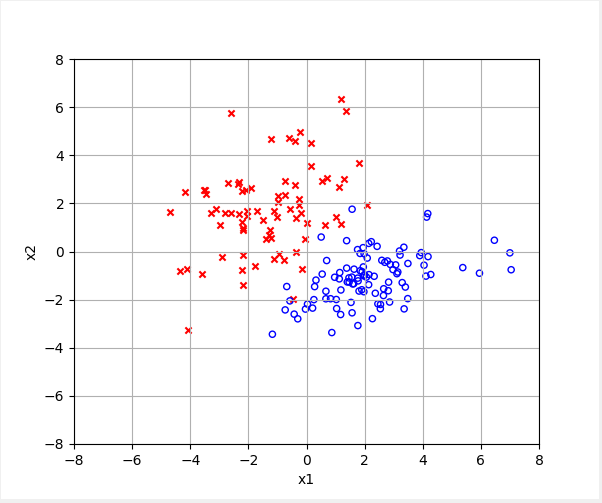
\includegraphics[width=0.5\textwidth]{../A1/aufgabe1C.PNG}
  \end{figure}

% Aufgabe 2

% Aufgabe 3

% Aufgabe 4



\end{document}
